\documentclass[reprint, onecolumn, amsmath, amssymb, showpacs, superscriptaddress, aps, prl]{revtex4-2}
\usepackage{fancyhdr} % Custom headers and footers
\pagestyle{fancyplain} % Makes all pages in the document conform to the custom headers and footers
\usepackage{setspace}
\pagenumbering{arabic} % Arabic/Indic page numbers

\usepackage{titlesec}
\doublespacing
\usepackage{microtype}% improves general appearance of the text
\usepackage{graphicx}% Include figure files
\usepackage{dcolumn}% Align table columns on decimal point
\usepackage{bm}% bold math
\usepackage{xcolor, soul}
\sethlcolor{red}
 \raggedbottom


\begin{document}
\title{Analyzing Trends in achieving World Sustainability Goals}

\author{Russu Anastasiia}



\begin{abstract}
This study will examine three important questions: the nature of the four trends of suitability development, the prediction of the low-carbon energy goals achievement, and school education trends. The question explores the trends of electricity access, equal representation of women and men in parliaments, internet access for all, and sufficient food for everyone, testing them for linearity and exploring polynomial trends for better prognosis. We want to offer suggestions through this study effort for tackling these issues and creating a sustainable future for everyone.
\end{abstract}


 \maketitle

\section{Introduction}
The Sustainable Development Goals (SDGs) of the United Nations were created to take care of everyone's fundamental human needs\cite{SchmidtTraub2018SDGIA}. These objectives include, among others, eradicating poverty, ensuring access to decent healthcare, and delivering quality education. UNICEF has established these objectives as a requirement for giving every child globally a healthy childhood\cite{20171423}.

This research examines how far the globe and a few particular nations have come in fulfilling the SDGs. The dataset spans from 2001 to 2018 and includes 12 sustainable development indicators that UNICEF has been tracking.

We analyze the linear behaviour of the trends. The presumption of linear growth in human achievements may be overly optimistic, so this study will examine nonlinear trends in data to provide a more accurate forecast of when the world and particular countries will achieve their goals. We have data for sustainable indicators for all countries. It is needed to be noted sometimes data is missing due to the goal achievement Objective of this research is to explore the data for the \(r^2\) and curve fit. 

\section{Analysis of the Linearity of the Trends}
To examine what type of trend better explains the behaviour of the data, we first explored the World Trends using two assumptions - about the linear and polynomial nature of the trends. Based on the original trend prediction lies the assumption about the linearity of the trend of reaching the sustainability goals, however, we should first check the correctness of it. As the measure of a good fit of the curve, we have used the Method of the Least Squares \cite{HESS20015211}. 
First of all, we explored the world trends for these four goals. We made comparisons between the years of the achievement of goals with linear and polynomial trends. The predicted years and the \(r^2\) for each goal can be seen in the table below. Coefficients of determination of the polynomial fit are equal to or better than the linear fit, however linear fit also has very high results.
\begin{table}[h!]
\begin{tabular}{lcccc}
                     & electricity & women & internet & undernourishment \\
linear               & 2045        & 2085  & 2035     & 2041             \\
\(r^2\) & 0.81        & 0.96  & 0.95     & 0.9              \\
polynomial           & 2025        & 2051  & 2026     & never            \\
\(r^2\) & 0.96        & 0.96  & 0.98     & 0.93            
\end{tabular}
\end{table}
\begin{figure}[h!]%
    \centering
    \subfloat{{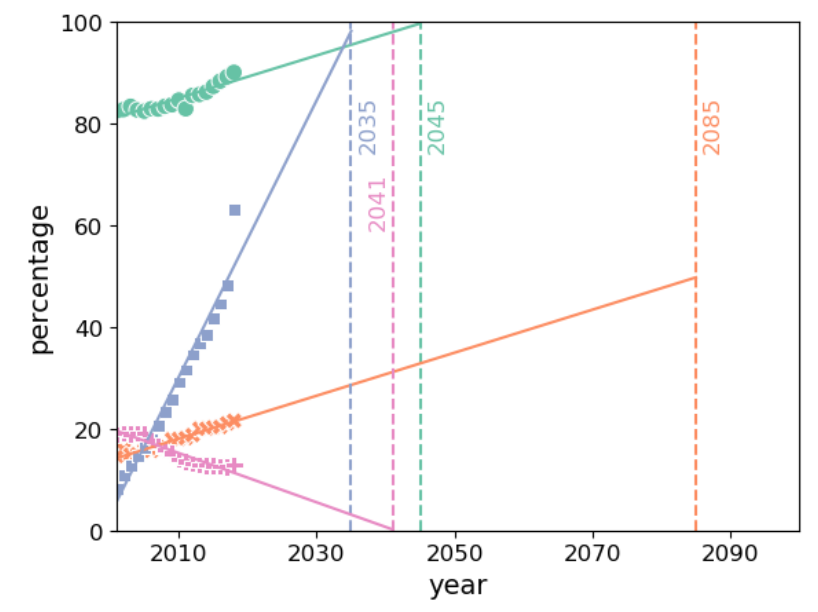
\includegraphics[width=7cm]{pictures/linear all oals.PNG} }}%
    \qquad
    \subfloat{{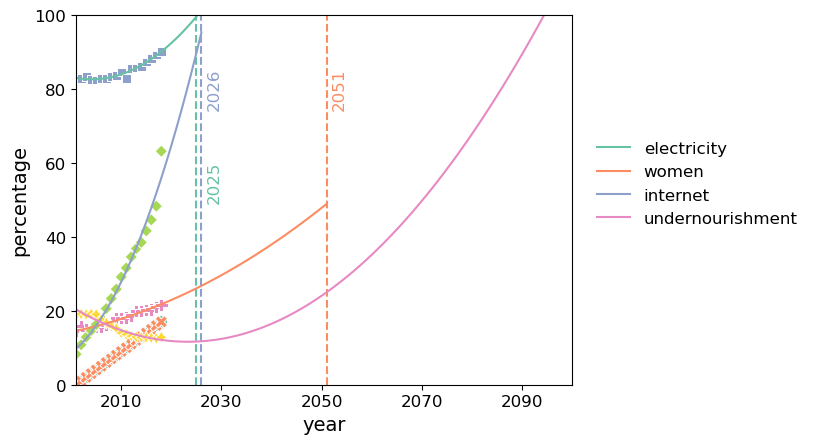
\includegraphics[width=9.5cm]{pictures/all the goals polynomial.png} }}%
    \caption{Prediction for the year of achievement the goal for linear and polynomial trend respective}%
    \label{fig:example}%
\end{figure}

We see that trend for the Internet exceeds the trend for available electricity by 10 years. In reality, it may be quite improbable as to use the internet one needs electricity. This kind of prediction happened, as the internet is a (relatively) recent invention and it is spread much faster than electricity. However, we can see this limit of linear trend prediction. 
On the other hand, the polynomial function makes less contradicting predictions about the use of the internet and electricity - consecutive years of 2025 and 2026. However, the flow of the polynomial model in the curve always goes up, and the goal of sufficient nutrition is never reached because of that. Also, the polynomial trend makes a more optimistic prediction for the equal representation of women in parliament - 2051 instead of 2086. 



As the most dramatic change in the \(r^2\) happens for the electricity, we will look closer at the data for this goal. The graph shows the linear and polynomial fit, \(r^2\) 0.81 and 0.96 respectively. For this case, the polynomial fit is quite successful, as \(r^2\) increases, while the prediction stays logically correct.  \footnote{the authors of this report are usually strongly committed to the beginning of the scale at 0. In this case, we consider it appropriate to use part of the scale for better visibility of data, as readers already had the chance to see the real scale of it.}

\begin{figure}[h!]%
    \centering
    \subfloat{{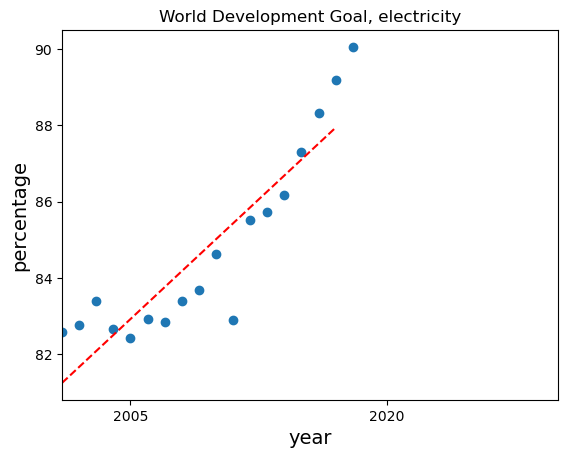
\includegraphics[width=8cm]{pictures/jfdk.png} }}%
    \qquad
    \subfloat{{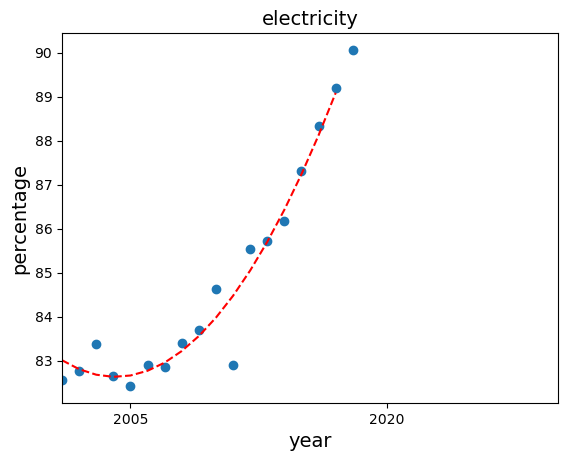
\includegraphics[width=8cm]{pictures/electricity_polynomial.png} }}%
    \caption{Prediction for the year of achievement the accessibility of the electricity for linear and polynomial trend respective}%
    \label{fig:example}%
\end{figure}

As the third step of the exploring linearity of the data, we will look at the goals and countries with the worst \(r^2\) for the linear fit. The countries with the worst linear fit are Tajikistan, Bulgaria, Niger and Liberia. For the goal of access to electricity, the worst result has Tajikistan with \(r^2\) = 0.027, however, the polynomial fit did not increase the score even for ten thousandths. The graph does not show a stable trend, so both curves work poorly in this case.
The same pattern in data we can see with the goal of equal representation of women in Bulgaria. The linear and polynomial fit \(r^2\) is equal to 0.00863.
\begin{figure}[h!]%
    \centering
    \subfloat{{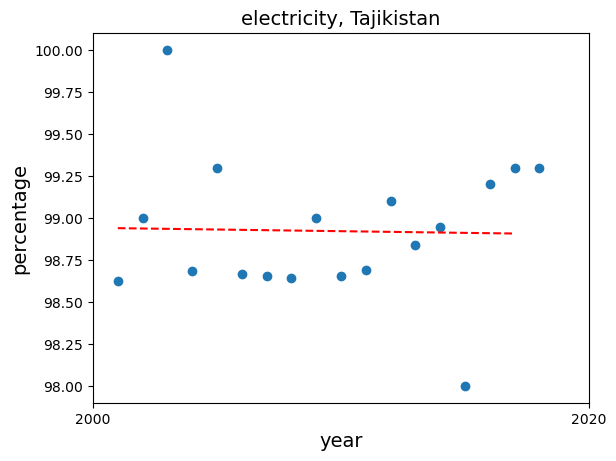
\includegraphics[width=8cm]{pictures/electricity Tadjikistan.png} }}%
    \qquad
    \subfloat{{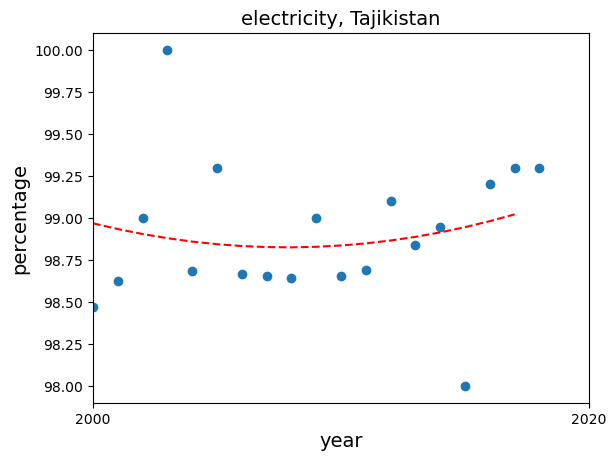
\includegraphics[width=8cm]{pictures/electricity Tadjikistan polynomia;.png} }}%
\end{figure}
\begin{figure}[]%
    \centering
    \subfloat{{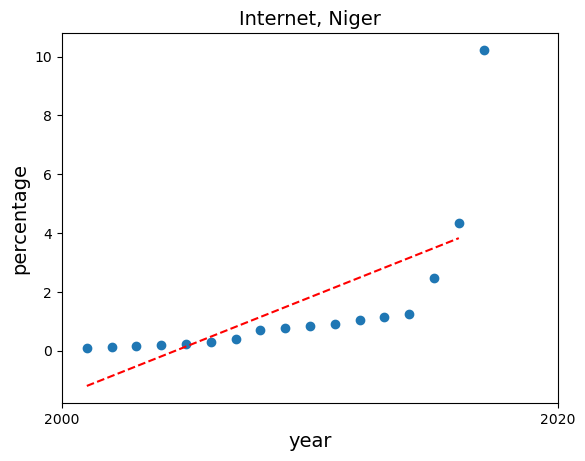
\includegraphics[width=8cm]{pictures/internet niger.png} }}%
    \qquad
    \subfloat{{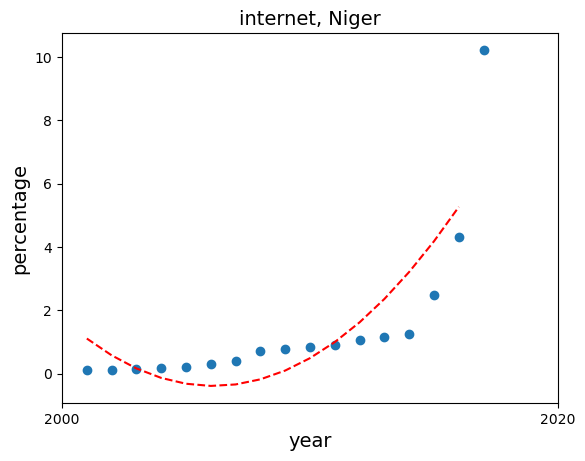
\includegraphics[width=8cm]{pictures/nih.png} }}%
\end{figure} 
\begin{figure}[]%
    \centering
    \subfloat{{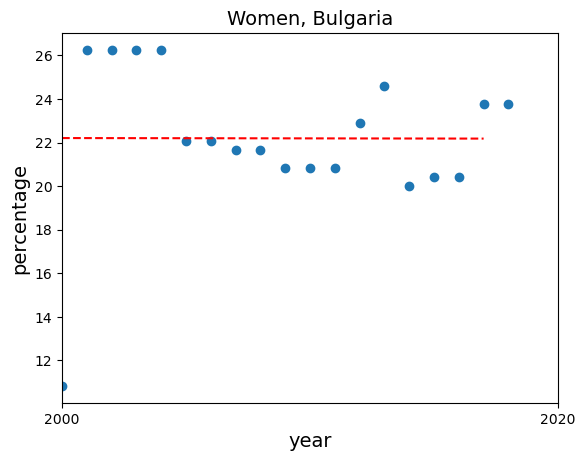
\includegraphics[width=8cm]{pictures/women bulgaria linear.png} }}%
    \qquad
    \subfloat{{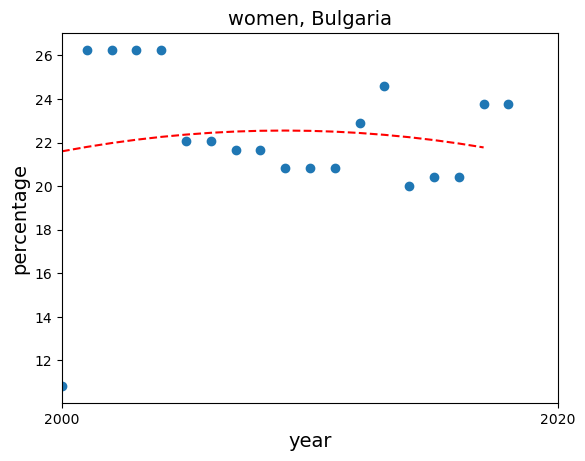
\includegraphics[width=8cm]{pictures/bulg.png} }}%

    \label{fig:example}%
\end{figure}
\begin{figure}[h!]%
    \centering
    \subfloat{{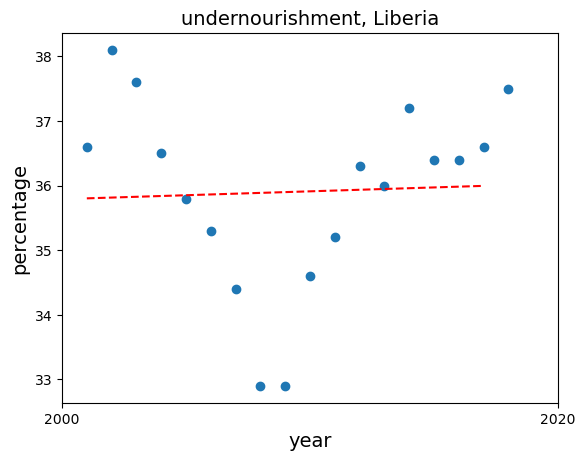
\includegraphics[width=8cm]{pictures/undernourishment Liberia linear.png} }}%
    \qquad
    \subfloat{{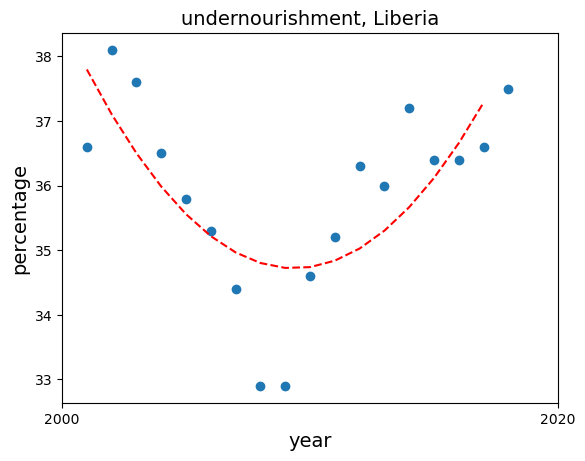
\includegraphics[width=8cm]{pictures/liberia pol.png} }}%
    \label{fig:example}%
\end{figure}

For the goal of equal access to the internet, Niger has \(r^2\) = 0.46. Looking at the data, we can see that for 15 years, Niger had very stable indicators around 1 percent of internet cover, and they began to grow around 2015 very quickly. The polynomial fit increases \(r^2\) to 0.72. 

The best improvement for polynomial fit among these four countries happened with Liberia, which scored 0.0019 with a linear fit. However, the score has increased to 0.545 with the polynomial curve. The data for this country has parabolic behaviour, which may be connected with the decrease in the level of life in the 2010s, probably economic crisis of 2008. 
In conclusion, in this part of the report, we examined data for the linear and non-linear trends. On the example of the average achievement for the whole world, we have seen that both linear and polynomial trends work with certain limitations: the linear trend was not logically comprehensive about access to the internet and electricity, while the polynomial trend fail to predict the year of the reach the goal of access to sufficient food. Coefficients of determination for both curve fit are high (around 90 percent), however overall the \(r^2\) scores of polynomial fit are higher. In the example of reaching the goal of accessible electricity, we have seen that \(r^2\) has risen from 81 per cent to 96, which means that in some cases polynomial curve may do better predictions. Nevertheless, in the instances of the worst linear \(r^2\) we have noticed the counterexamples when the use of the polynomial curve did not improve the results. Finally, the assumption of the nature of any kind of trend should be reviewed before the implementation of it into prediction. 


\section{Conclusion}

One of the important limitations of the study is the different quality of the data for different countries. Though UNICEF tries to provide the best available data, some countries consistently drop out of the research because of the lack of data. This is one of the big vicious circles of the countries without working institutions, as in order to fix the problems that UNICEF addresses, good-quality data is needed, however, countries cannot provide it because of the exactly these problems. 

We have explores the linearity of the world trends of four SDG goals and found out that the overall polynomial curve better fits the data, however, both linear and non-linear trends have mathematical and logical limitations in use. For the worst cases of coefficients of the determination for the linear fit, we have investigated the polynomial one and concluded they both may not work on certain types of data. Potentially, other kinds of functions may be explored for better fit and more accurate and consistent predictions. Also, the paths of the other countries that already achieved the goals may be studied, as for now they were excluded from the analysis if they have reached their goals before 2001 \cite{diaz2018sustainable}. 


The findings of this study can influence national policies and programs that promote sustainable energy practices and direct private-sector decision-making toward more ethical and sustainable business practices. In addition, the goal of the research on the SDG is into providing trustworthy and credible research findings that support international efforts to lower carbon emissions and build a more sustainable future by applying a strict approach to data cleaning and formatting.

\bibliographystyle{plain}    % The bibliography style. This is plain but it can be changed depending on your preference
\bibliography{1, citation,scholar,2}    % The file name of the .bib file

\end{document}